% !TEX TS-program = pdflatex
\documentclass[11pt,a4paper]{article}

% Use TeX-distributed Type 1 fonts so arXiv does not depend on host fontconfig.
% Helvetica is metrically close to Arial; the generated charts embed Arial.
\usepackage[T1]{fontenc}
\usepackage[scaled=0.95]{helvet}
\usepackage{courier}
\renewcommand{\familydefault}{\sfdefault}
\setlength{\emergencystretch}{2em}

\usepackage[a4paper,margin=23mm,headheight=15pt]{geometry}
\usepackage{amsmath,amssymb}
\usepackage{booktabs,longtable,tabularx,array,multirow}
\usepackage{graphicx}
\usepackage{xcolor}
\usepackage{enumitem}
\usepackage{fancyhdr}
\usepackage{listings}
\usepackage{caption}
\usepackage{tikz}
\usetikzlibrary{arrows.meta,positioning,fit,shapes.geometric}
\usepackage{hyperref}
\usepackage[nameinlink,noabbrev]{cleveref}

\definecolor{mfblue}{HTML}{2F5D8C}
\definecolor{mfteal}{HTML}{2A8C82}
\definecolor{mforange}{HTML}{D17A3A}
\definecolor{mfred}{HTML}{B44A4A}
\definecolor{ink}{HTML}{25313C}
\definecolor{codebg}{HTML}{F5F7FA}
\hypersetup{
  colorlinks=true,
  linkcolor=mfblue,
  urlcolor=mfblue,
  citecolor=mfteal,
  pdftitle={DeepSeek-V4-Flash on AMD gfx90a: Correctness and Performance Engineering},
  pdfauthor={Media Foundry / SGLang gfx90a Engineering}
}

\lstdefinestyle{reportcode}{
  basicstyle=\ttfamily\small,
  backgroundcolor=\color{codebg},
  frame=single,
  rulecolor=\color{black!15},
  breaklines=true,
  columns=fullflexible,
  keepspaces=true,
  showstringspaces=false,
  upquote=true
}
\lstset{style=reportcode}

\newcolumntype{Y}{>{\raggedright\arraybackslash}X}
\newcommand{\metric}[1]{\textbf{\color{mfblue}#1}}
\newcommand{\risk}[1]{\textbf{\color{mfred}#1}}
\newcommand{\commit}[1]{\texttt{#1}}

\pagestyle{fancy}
\fancyhf{}
\fancyhead[L]{DeepSeek-V4-Flash on AMD gfx90a}
\fancyhead[R]{Technical report v0.3}
\fancyfoot[C]{\thepage}

\title{\bfseries DeepSeek-V4-Flash on AMD gfx90a\\[3mm]
\Large Correctness Recovery and Inference Performance Engineering}
\author{Media Foundry / SGLang gfx90a Engineering}
\date{September 14, 2026\\[1mm]
\small TP8 matrix archive \commit{3d73a75923}; native-AR pilot \commit{fb2e39fca9}}

\begin{document}

\maketitle

\begin{abstract}
We report the enablement, correctness recovery, and performance engineering of DeepSeek-V4-Flash inference on AMD Instinct MI250 (gfx90a/CDNA2) using SGLang. Original mixed FP4/FP8 checkpoint weights are retained; execution uses shape-specific HIP, AIter, Composable Kernel, and Triton paths. The study extends an earlier four-GCD investigation to a single eight-GCD tensor-parallel instance with a 1,048,576-token logical KV pool. Fresh-process native autoregressive measurements on public-source code requests cover concurrency 1 through 64, with three measured rounds per group. Single-request resident decode reaches \metric{87.60 output tokens/s}, while C32 and C64 reach \metric{1044.32} and \metric{1334.24 output tokens/s}. Separate 8K-input prefill measurements span \metric{4.68--5.27k input tokens/s}. An exact empty-indexer-tile guard provides a 3.60-fold resident improvement in a separate 8K-input C32 ABBA test; a restored single-request projection specialization improves its matched control by 10.32\%. A subsequent, default-off down-consumer pilot adds 1.54\% at C32. We distinguish these workload-specific results from historical speculative throughput and from whole-request HTTP latency. Component equality and bounded semantic checks do not establish universal numerical equivalence; dynamic batching, cold-shape compilation, and untested million-token occupancy remain explicit limitations.
\end{abstract}

\tableofcontents
\clearpage

\section{Executive summary}

\begin{table}[htbp]
  \centering
  \caption{Evidence-backed state as of September 14. C denotes client concurrency; resident decode excludes admission and drain.}
  \label{tab:headline}
  \begin{tabularx}{\textwidth}{@{}p{0.29\textwidth}Y@{}}
    \toprule
    Item & Result \\
    \midrule
    Model & DeepSeek-V4-Flash; 284B total parameters, approximately 13B active parameters, FP4 routed experts, and mostly FP8 non-expert weights \\
    Host platform & Supermicro A+ Server AS-4124GQ-TNMI; dual AMD EPYC 7763 processors with SMT enabled; 1 TiB DDR4-2933 from 32 $\times$ 32 GiB 2Rx8 RDIMMs \\
    Accelerators & Eight MI250 GCDs (gfx90a), approximately 64 GiB HBM per GCD; four dual-GCD accelerators, not eight MI250 boards \\
    Formal native decode & C1 87.60; C32 1044.32; C64 1334.24 resident output tok/s; full seven-tier table in \cref{tab:tp8-matrix} \\
    Formal prefill & 8K public-source inputs: 4676.39--5265.43 input tok/s across C1--64; admission limited to 16 requests \\
    Additional C32 pilot & 1044.61$\rightarrow$1060.70 resident tok/s (+1.54\%); opt-in, separate corpus protocol, not a replacement matrix cell \\
    KV pool & 1,048,576 logical tokens allocated; no filled-1M-context performance or quality certification \\
    Runtime topology & One TP8/EP1 instance, no routed-expert A2A; native decode graph tiers 1/2/4/8/16/32/64 \\
    Service state & Benchmark services stopped after testing; no live endpoint is implied by this report \\
    \bottomrule
  \end{tabularx}
\end{table}

The report applies three evidence rules:

\begin{enumerate}[leftmargin=2em]
  \item Native AR, full-target DSpark, and historical approximate-target DSpark are different experiments. Their rates are not interchangeable.
  \item Original checkpoint precision, component equality, repeated output hashes, and end-to-end answer quality are distinct claims. No one check substitutes for the others.
  \item Formal three-round matrices and small ABBA screens remain separate. Minima/maxima describe observed runs, not confidence intervals; percentages from different experiments are not added together.
\end{enumerate}

\section{Related systems}

This work builds on serving systems that reduce scheduling and memory-management overhead for autoregressive language models. SGLang combines a structured runtime with RadixAttention and continuous batching, while vLLM introduced PagedAttention to manage KV-cache fragmentation and sharing efficiently\cite{sglang,vllm}. Our contribution is narrower and hardware-specific: we retain SGLang's serving abstractions while adapting the DeepSeek-V4 execution path to CDNA2 and validating optimizations against fixed-token numerical oracles.

DeepSeek-V3 established the MoE, routing, multi-token prediction, and low-precision training lineage; DeepSeek-V4 adds compressed sparse/heavily compressed attention and mHC\cite{dsv3,dsv4report}. MegaBlocks demonstrates block-sparse MoE training\cite{megablocks}; our serving workload instead spans tiny per-expert decode matrices and large prefill chunks. These regimes require different execution geometries rather than a universal kernel. DSpark supplies a separate confidence-scheduled speculative design\cite{dspark}; we report its historical full-target results separately from the current native-AR matrix.

On AMD GPUs, Composable Kernel and AIter provide tuned HIP, CK, and CKTile building blocks for GEMM, quantization, attention, and MoE\cite{ck,aiter}. We use these libraries where their supported shapes are effective, but introduce gfx90a-specific paths where generic kernels do not match FP4 storage, wave64 execution, or the small-$M$ decode regime. The resulting system is therefore an integration and measurement study rather than a replacement for either the serving runtime or the kernel libraries.

\section{System and model context}

\subsection{Hardware and software stack}

The experimental host is a Supermicro A+ Server AS-4124GQ-TNMI with two AMD EPYC 7763 processors and SMT enabled. Host memory comprises 32 32-GiB DDR4-2933 2Rx8 RDIMMs, totaling 1 TiB. Historical TP4 runs used four GCDs; the new TP8 matrix uses all eight GCDs as one model instance, not two independent TP4 replicas. The accelerators are MI250, not MI250X.

The September environment record identifies Python 3.12.13, PyTorch \texttt{2.12.0a0+git78258b9}, Triton \texttt{3.7.1+git0263a6a6.rocm7.14.0}, Transformers 5.12.1, and Tokenizers 0.22.2. The installed HIP compiler reports 7.15.26333 and AMD clang 23; this is distinct from the HIP 7.14 build provenance recorded in earlier runs and does not identify every cached binary. SGLang, AIter, and CK include local source changes. The environment ledger lists dependency commits and dirty paths; a clean SGLang commit alone is not a complete binary reproducibility guarantee.

The original checkpoint comprises 48 indexed safetensors shards. Recorded SHA256 values cover configuration, tokenizer, generation settings, and the shard index, not every weight byte. This study does not include V4.1 or Engram offload results.

CDNA2 provides wave64 execution, 64 KiB LDS per CU, and INT8/BF16/FP16 matrix or dot instructions, but no native FP4 matrix core comparable to newer accelerator generations. DeepSeek-V4-Flash stores routed-expert weights in FP4. Consequently, the critical gfx90a cost is not raw HBM bandwidth alone: it is the combination of small-M utilization, online FP4 unpacking, scale handling, activation quantization, expert sorting, and layer-level synchronization. The AMD MI200 ISA manual guided the custom HIP kernels in this work\cite{amdisa}.

\subsection{Execution structure}

DeepSeek-V4-Flash has 43 decoder layers, 256 routed experts, top-6 routing per token, shared experts, mHC, and compressed sparse attention. The official model card reports 284B total parameters, 13B active parameters, a one-million-token context, and mixed FP4 expert / FP8 non-expert precision\cite{dsv4card}.

\begin{figure}[htbp]
  \centering
  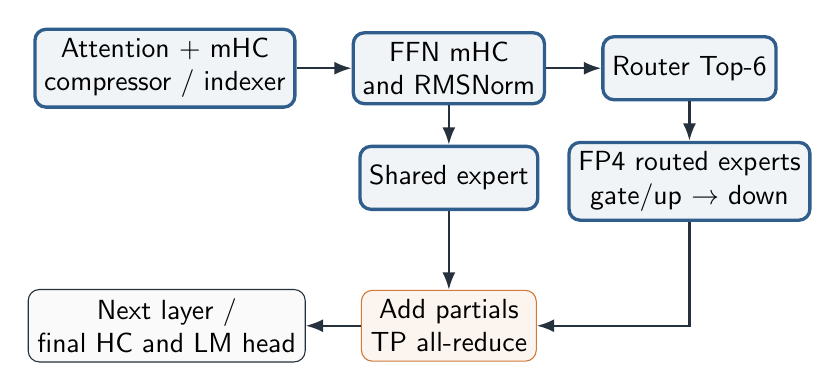
\begin{tikzpicture}[
    node distance=5mm and 7mm,
    box/.style={draw=ink,rounded corners,align=center,minimum height=8mm,fill=black!2},
    hot/.style={draw=mfblue,very thick,rounded corners,align=center,minimum height=8mm,fill=mfblue!7},
    comm/.style={draw=mforange,rounded corners,align=center,minimum height=8mm,fill=mforange!8},
    arrow/.style={-{Latex[length=2.2mm]},thick,color=ink}
  ]
    \node[hot] (attn) {Attention + mHC\\compressor / indexer};
    \node[hot,right=of attn] (ffn) {FFN mHC\\and RMSNorm};
    \node[hot,right=of ffn] (router) {Router Top-6};
    \node[hot,below=of router] (routed) {FP4 routed experts\\gate/up $\rightarrow$ down};
    \node[hot,below=of ffn] (shared) {Shared expert};
    \node[comm,below=10mm of shared] (reduce) {Add partials\\TP all-reduce};
    \node[box,left=of reduce] (head) {Next layer /\\final HC and LM head};
    \draw[arrow] (attn) -- (ffn);
    \draw[arrow] (ffn) -- (router);
    \draw[arrow] (router) -- (routed);
    \draw[arrow] (ffn) -- (shared);
    \draw[arrow] (routed.south) |- (reduce.east);
    \draw[arrow] (shared) -- (reduce);
    \draw[arrow] (reduce) -- (head);
  \end{tikzpicture}
  \caption{Schematic native TP-only layer boundaries. Shared and routed experts contribute to a join. TP4/EP1 and TP8/EP1 avoid expert A2A but retain TP collectives; the historical EP variants instead require dispatch/combine.}
  \label{fig:architecture}
\end{figure}

\section{gfx90a enablement}

The original ROCm path primarily targeted gfx942 and gfx950. The gfx90a bring-up required the following changes:

\begin{itemize}[leftmargin=2em]
  \item add gfx90a as a build target and select \texttt{HIP\_FP8\_TYPE\_FNUZ};
  \item repair ROCm 7.14 include, library, and rpath discovery while avoiding the conda host-side \texttt{hipcc};
  \item build AOT HIP kernels and enable AIter FP4 CK MoE execution on gfx90a;
  \item handle Mori topology and XGMI initialization on a node without an RDMA NIC;
  \item validate HIP CUDA Graph capture and replay on gfx90a instead of attributing architecture-specific kernel selection failures to the hardware;
  \item establish both TP4/EP4 with Mori and TP4/EP1 without A2A as executable reference paths.
\end{itemize}

The initial bring-up checkpoint was \commit{505b3373794a}. It predates the later correctness and performance work and must not be treated as the final state.

\section{Correctness recovery}

\subsection{Admission, sampling, and chat encoding}

An early request stall was an SWA admission failure rather than a Mori or RCCL deadlock. The combination of \texttt{max-total-tokens=4096}, \texttt{swa-full-tokens-ratio=0.1}, and \texttt{page-size=256} produced a pool below the admission floor. A separate gfx90a AIter greedy-sampler issue could return \texttt{token\_id == vocab\_size} on special logits rows; gfx90a now uses \texttt{torch.argmax} for this case.

DeepSeek-V4 does not ship a Jinja chat template. It requires the model-specific encoding and output parser, which is also stated in the official model card\cite{dsv4card}.

\subsection{W2 permutation: invalidating the early 60 tok/s result}

\risk{The early approximately 60 tok/s AIter FP4 route was not correctness-valid.} The legacy CK FP4-by-FP4 stage-1 path produced zeros on gfx90a. After switching to CKTile BF16-by-FP4, stage 1 reached approximately 0.999996 cosine similarity to a direct oracle, but stage-2 W2 remained near 0.24.

Output-column fingerprinting identified the following 16-row block mapping within each 128-wide N tile:

\begin{equation}
  \text{fast}\rightarrow\text{reference}=[0,2,4,6,1,3,5,7].
\end{equation}

Applying the inverse permutation

\begin{equation}
  [0,4,1,5,2,6,3,7]
\end{equation}

to raw W2 weights and scales during loading restored the logical output order for top-k=1 and top-k=6. This is a one-time load transformation with no decode hot-path cost.

The fixed France oracle uses the following input IDs:

\begin{lstlisting}
[0,128803,3085,344,270,6102,294,8760,2755,128804,128822]
\end{lstlisting}

Its expected completion is:

\begin{lstlisting}
The capital of France is **Paris**.
token ids: [671,6102,294,8760,344,2619,51119,42499,1]
hash: 6f41fe2f01d52507
\end{lstlisting}

The short sentinel was stable in the documented eager, graph, and independent-start checks. This bounded test cannot certify a long context, a different batch shape, or the entire numerical pipeline. Greedy completions can diverge from the first token under different prefill execution; fixed-input logits and layer comparisons are needed to locate such differences.

\subsection{Later numerical and integration repairs}

The later investigation also identified an independent E8M0 scale-layout issue in large-prefill BF16-CK execution: raw packed weights do not imply raw logical scales. Runtime AIter scale shuffling must be inverted or consumed with the matching address map. Constant-scale synthetic fixtures can hide this error. Selected CK paths still use FP32 atomic accumulation; layout repair does not make their reduction order deterministic.

Deterministic index selection fixes membership ties using logical IDs and presents selected positions in a fixed order before rank-local physical mapping. The prefill trivial-row shortcut retains real sequence lengths and all compressor/cache updates; only scores irrelevant to Top-K are skipped. Subsequent native-decode empty-tile elimination is a separate optimization, described in \cref{sec:current-native}.

Fresh starts after the upstream/V4.1 integration exposed missing C4 lifecycle callbacks and incorrect compression-ratio discovery for unified V4 pools. Their repair restored the requested logical 1M pool and native graph construction. CPU tests also cover SWA-only draft metadata, but the latest user scope excluded DSpark: the completed native matrix is not a fresh DSpark GPU validation.

\section{Historical TP4 decode optimization}

\subsection{Parallel decomposition}

After the W2 repair, the corrected TP4/EP4+Mori BS1 baseline was only 14.2--15.0 tok/s. The TP4/EP1 no-A2A CKTile reference reached approximately 20.14 tok/s. This comparison motivated investigation of dispatch/combine, rank imbalance, and progress overhead; changing the expert decomposition also changes compute shapes, so it does not isolate communication cost.

The historical TP4/EP1 decode route combines:

\begin{itemize}[leftmargin=2em]
  \item packed 4-bit FP4 weights without an offline expansion;
  \item online BF16 activation quantization to INT8 per 32 elements;
  \item E2M1 nibble mapping to $0,\pm1,\pm2,\pm3,\pm4,\pm6,\pm8,\pm12$;
  \item CDNA2 \texttt{v\_dot4\_i32\_i8} / mixed-dot accumulation followed by activation and E8M0 scaling;
  \item four 16-lane subgroups for top-6 slots in the down projection;
  \item AIter peer-read custom all-reduce in place of the high fixed-latency RCCL path;
  \item TP-only mHC launch geometry that no longer reserves CUs for Mori progress.
\end{itemize}

\begin{figure}[htbp]
  \centering
  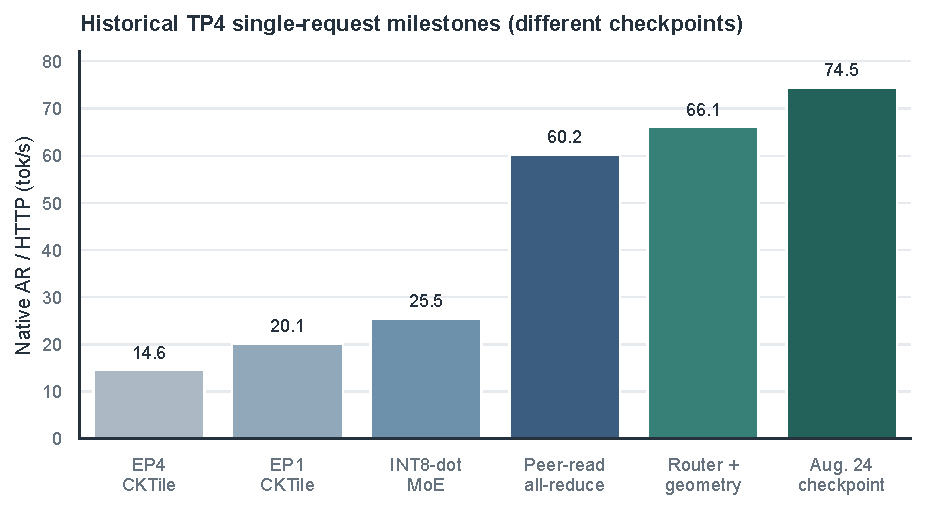
\includegraphics[width=0.96\textwidth]{figures/decode_progress.pdf}
  \caption{Historical TP4 short-probe milestones retained from the earlier report. Different checkpoints and controls are not a single controlled speedup series. The invalid early FP4 route is excluded; the later 60.20 point follows a separate repair.}
  \label{fig:decode-progress}
\end{figure}

The ledger associates the largest jump in \cref{fig:decode-progress} with peer-read all-reduce, approximately 25.54 to 60.20 tok/s. The August short-probe milestone is about 74.5 tok/s. A September 6 isolated-tree reproduction obtained a seven-request HTTP median of 74.018 and maximum of 74.655 tok/s, with the historical hash on all seven requests. This was \emph{TP4 native AR}, not TP8 or DSpark. The inherited rebased tree ran about 53 tok/s; its different tree contents exposed a lost gfx90a MHC selector. Historical author dates and copied experiment notes did not establish performance on the rebased code. The current TP8 C1 result uses a different public-code protocol and must not be divided by 74.5 to claim TP scaling efficiency.

\section{Prefill optimization and historical checkpoints}

\subsection{From per-assignment scalar work to CDNA2 MFMA}

The original raw-FP4 direct kernel sent M=256 prefill through a per-assignment FP16 dot path, with approximately 12.9 s TTFT for a 1028-token prompt. The optimization sequence introduced:

\begin{enumerate}[leftmargin=2em]
  \item packed-FP4 unpack reuse across rows, first group8 and then group32 for M$\geq$1024;
  \item \texttt{v\_perm\_b32} lookup tables instead of branch-heavy nibble decoding;
  \item MI250 block-FP8 tuned configurations for M512 and M1024 dense projections;
  \item CDNA2 INT8 MFMA routed gate and down kernels;
  \item sparse paged-prefill attention reduction from eight waves to one wave;
  \item chunked-prefill growth from 512/1024 to 2048;
  \item M2048-specific MFMA grids, native HIP INT8 quantization, and scale/metadata broadcast;
  \item an expert sorter block increase from 32 to 64 rows, allowing an expert with approximately 48 assignments to scan packed weights once.
\end{enumerate}

\begin{figure}[htbp]
  \centering
  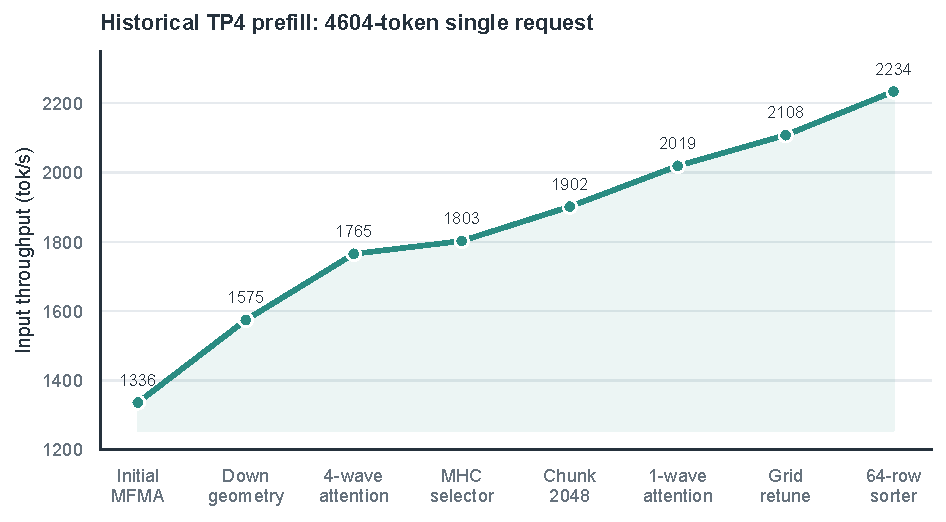
\includegraphics[width=0.96\textwidth]{figures/prefill_progress.pdf}
  \caption{Historical TP4 sequence for a 4604-token prompt. Rates derive from HTTP TTFT; these points are not the latest 8K-input TP8 matrix.}
  \label{fig:prefill-progress}
\end{figure}

The historical M2048 microbenchmark compares the 32-row and 64-row sorter variants in \cref{fig:micro}. Gate/up improves from 7.26 to 5.55 ms (23.6\%), down improves from 6.01 to 5.26 ms (12.5\%), and the combined kernel time improves by approximately 18.5\%. The recorded component fixtures reported identical outputs; this is not a full-model equality claim.

\begin{figure}[htbp]
  \centering
  \begin{minipage}[t]{0.49\textwidth}
    \centering
    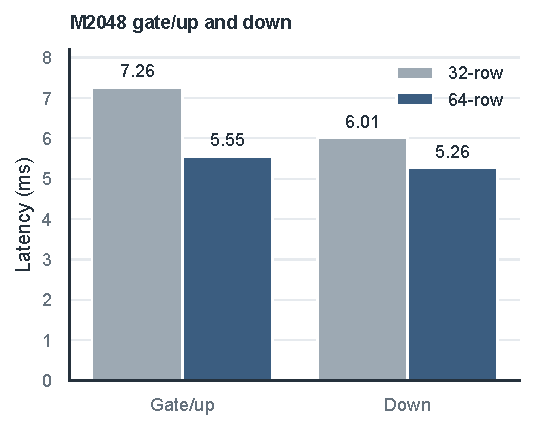
\includegraphics[width=\linewidth]{figures/moe_microbenchmark.pdf}
  \end{minipage}\hfill
  \begin{minipage}[t]{0.49\textwidth}
    \centering
    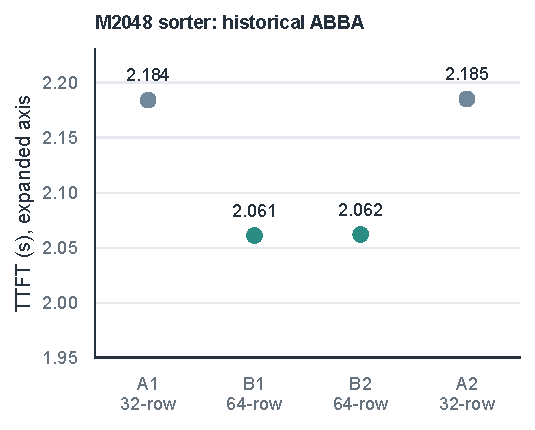
\includegraphics[width=\linewidth]{figures/prefill_abba.pdf}
  \end{minipage}
  \caption{Left: M2048 routed-MoE kernel latency. Right: strict endpoint-level ABBA validation of the 64-row sorter.}
  \label{fig:micro}
\end{figure}

The historical endpoint ABBA sequence was A1=2.184 s, B1=2.061 s, B2=2.062 s, and A2=2.185 s. A later chunk-only TP4 test used B1=1.861 s, A=1.978 s, and B2=1.852 s (six steady samples per arm). Chunk 2304 removes the small tail traversal for 4604 tokens; it is not a universal optimum over prompt lengths. The first new-shape request still took over 20 s, whereas the warm measurements were near 1.85 s.

\subsection{Large-M CK and the meaning of the earlier 6.42k result}

The subsequent BF16-CK prefill route materializes the current expert shard in BF16, runs CK stages, and casts the accumulated output back to BF16. It does not alter the checkpoint files, but changes execution arithmetic relative to raw-FP4/INT8-dot kernels. In the September 7 TP8 migration, 32 distinct requests totaling 73,724 input tokens, admission 16, and two approximately M36864 forwards reached a warm median of 6420.39 input tok/s with a 131,072-token pool. This is an aggregate prefill wave, not single-request decode. The latest matrix instead uses approximately 8K input per request and a 1M pool. Its 4.68--5.27k results do not by themselves prove a regression from 6.42k; length, pool, grouping, and timing differ.

\section{Current TP8 native-AR results}
\label{sec:current-native}

The primary result is the September 13--14 fresh-process revalidation on the
merged original-V4 implementation, archived at \commit{3d73a75923}. All seven
native graph tiers were captured and observed with matching active input and
executed rows during full residency. The model remained a single TP8/EP1
instance. No DSpark, MTP, or approximate routed-expert verification contributed
to the following table.

\begin{table}[htbp]
  \centering
  \caption{Formal native P/D matrix: P and resident D are three-round medians;
  HTTP aggregates complete measured waves. Prefill divides aggregate input by
  wave time to the last first token. Resident and HTTP decode are distinct metrics.}
  \label{tab:tp8-matrix}
  % Generated from data/results.json by prepare_report_data.py.
\begin{tabular}{@{}rrrr@{}}
\toprule
C & Prefill input tok/s & Resident output tok/s & HTTP output tok/s \\
\midrule
1 & 4676.39 & 87.60 & 86.39 \\
2 & 4989.25 & 109.94 & 102.41 \\
4 & 5265.43 & 188.71 & 148.50 \\
8 & 5099.23 & 334.18 & 254.45 \\
16 & 5171.36 & 608.23 & 422.51 \\
32 & 5254.98 & 1044.32 & 680.61 \\
64 & 5250.05 & 1334.24 & 848.14 \\
\bottomrule
\end{tabular}

\end{table}

\begin{figure}[htbp]
  \centering
  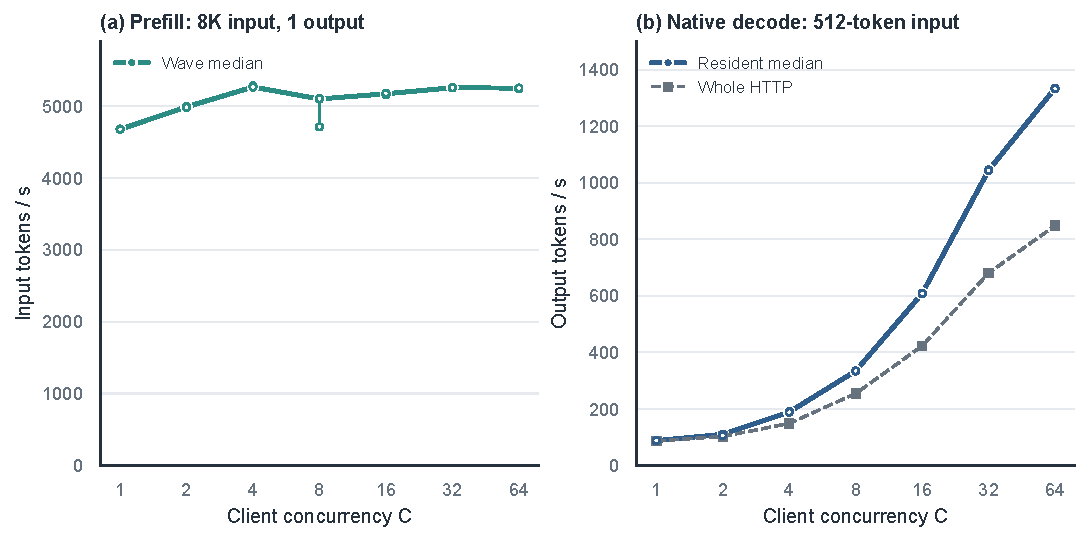
\includegraphics[width=\textwidth]{figures/tp8_pd_matrix.pdf}
  \caption{Latest TP8 matrix. Colored points/lines show three-round medians;
  thin vertical ranges and small points are actual rounds, not confidence
  intervals. Gray decode points are complete-wave HTTP rates, not a slower
  kernel configuration. Concurrency uses a base-2 axis.}
  \label{fig:tp8-pd}
\end{figure}

\paragraph{Protocol boundaries.}
Prefill uses 8191--8192-token public-source prompts, fresh cache salts, and one
output token. At C64 the wave contains about 524k input tokens, admitted at
most 16 requests at a time with a 36,864-token chunk budget. C64 therefore does
not mean one M64 prefill kernel or 64 simultaneous large prefill requests.
Decode uses 511--512-token inputs, greedy sampling, natural EOS, and at most
2048 output tokens. Each formal round accumulates at least 30 s of common
resident windows; explicit warmups are excluded. The 64-case corpus extends
the earlier 32-case public-source corpus without changing those first 32 cases.
Duration-dependent wave counts can expose different case mixtures, which are
preserved in raw records.

\paragraph{C1 supplement.}
The seven-tier run originally omitted the existing C1-only wo\_a GEMV opt-in.
It was restored, independently tested, and measured for three new C1 rounds.
The C1 row above uses that supplement. C2--64 resident windows cannot select
the M1 kernel; their whole-wave HTTP numbers nevertheless retain the measured
GEMV-off drain behavior. We do not claim a newly measured all-on HTTP matrix.

\paragraph{Interpretation.}
Prefill plateaus near 5.2k aggregate input tok/s under this admission/chunk
policy. Decode continues scaling through C64, reaching 1334.24 resident output
tok/s, but complete-wave throughput is 848.14 tok/s. The gap includes admission,
prefill, uneven answer lengths, and drain. It is not a measured host-only
overhead term. The C8 prefill rounds include 4710.94 alongside approximately
5100 input tok/s; this slower measured round is retained, not silently trimmed.
No matched current TP4 seven-tier matrix is available in the retained evidence,
so a TP4-to-TP8 scaling factor is not reported.

\subsection{Empty C4 tiles: pool capacity is not active context}

With a 1M logical pool, the C4 logits launch could cover 262,144 key positions
even when only a short prefix was active. Beyond the raw-token threshold near
2048, many launched tiles had no valid keys but still performed unnecessary
query loading and dot work. The exact native-decode guard skips this empty
work while retaining defined zero stores, unchanged active computation,
sequence lengths, Top-K semantics, and physical index mapping.

Seven component shapes, 100 mutations per shape, and 1000 graph replays per
shape checked score bits and logical/physical indices. Fully populated control
cases did not exhibit the empty-work benefit. At M32, the diagnostic component
dropped from approximately 6934 to 837 microseconds; this is not a whole-model
speed prediction.

A separate matched 8K-input C32 service ABBA measured
169.657 / 611.103 / 610.853 / 169.843 resident output tok/s, a 3.599-fold
candidate/control ratio. Complete HTTP rates were approximately 83.18 / 128.85 /
128.88 / 83.26 tok/s. The different ratios illustrate why the measurement
boundary must be explicit. This 8K test is not the 512-input formal decode
table, and its multiplier must not be applied to that table. This fix is
native-decode scoped; the earlier prefill trivial-row skip is a different path.

\subsection{Recovering the existing C1 projection specialization}

The restored wave64 wo\_a GEMV measured 30.75$\rightarrow$6.88 microseconds in
its component test. All 100 tested mutations were finite and repeatable, but
only 70 were bit-equal to the former einsum path; the maximum relative L2
error against a float32 reference was about 0.00179 on the test inputs.
It retains checkpoint weights while changing floating reduction.

The service ABBA was 79.558 / 87.583 / 87.504 / 79.151 resident output tok/s:
+10.32\% by mean candidate/control arms. Candidate repeats had identical
completion sequences in that test, and France passed. The separate formal C1
median is 87.599. These controls are more informative than an unpaired
comparison with the August 74.5 HTTP result.

\begin{figure}[htbp]
  \centering
  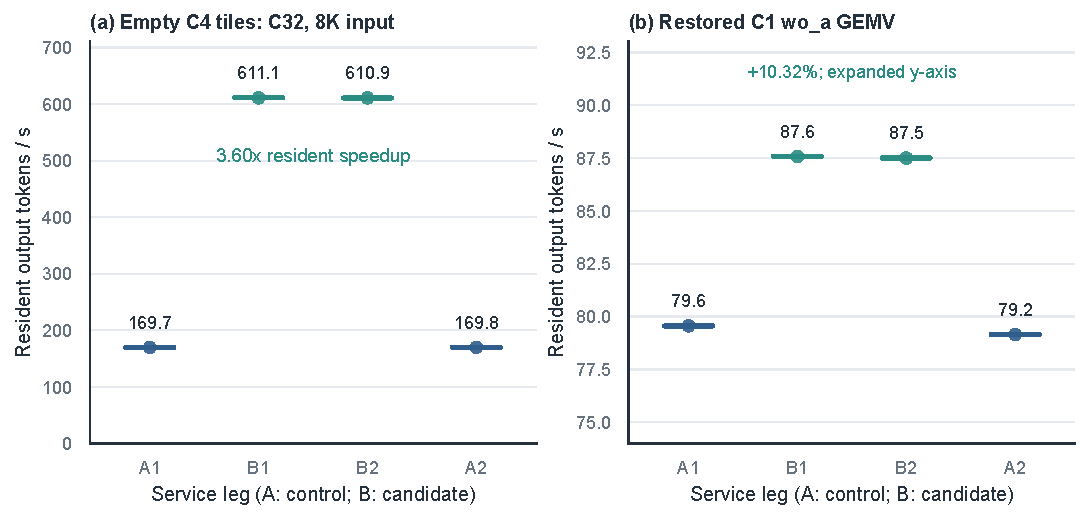
\includegraphics[width=\textwidth]{figures/native_abba.pdf}
  \caption{Separate native ABBA experiments: empty C4 tiles at C32 with 8K
  inputs, and the C1 projection specialization with 512-token code inputs.
  The right axis is expanded; the experiments must not be multiplied together.}
  \label{fig:native-abba}
\end{figure}

\subsection{Down-consumer pilot: a small C32 gain, no C1 kernel change}

The follow-up at \commit{fb2e39fca9} replaces the M32 second quantization/down
chain with a CTA16 consumer. Each CTA reads the already-rounded BF16
intermediate, forms group32 INT8 values/scales in LDS, computes its output
stripe, and retains the existing FP32 top-k partial and fixed reduction.
The current gate, sorter, original weights, attention, and TP collectives are
unchanged. The selector is limited to native TP8/EP1, M32/I256 and A4/R2
geometry; it remains default-off.

On one GCD, synthetic diverse/skewed inputs reduced quant+down+reduction from
130.542 to 115.907 microseconds and 81.615 to 70.791 microseconds, respectively.
Each distribution passed 100 mutations of inputs, routes, weights and scales
and 1000 checked graph replays. Comparisons used numeric element equality,
not a signed-zero-bit check. This is neither the full routed stage nor a
captured real-layer oracle.

The service screen uses two natural-EOS waves per leg with the same 32 code
requests, rather than the duration-driven formal 64-case protocol. C32 leg
medians are 1047.763 / 1060.206 / 1061.203 / 1041.459 resident tok/s. Mean
control 1044.611 versus candidate 1060.705 gives +1.541\%; the return control
changes $-0.602\%$, and candidate legs differ 0.094\%. Every candidate wave
exceeds every control wave. Whole HTTP rates vary with answer length and do
not establish the same percentage gain.

The conditional C1 test is an isolation check, not an M1 port: the existing
direct M1 down kernel already quantizes in LDS, with a different rounding
contract. Its control/candidate means are 89.722/90.024 tok/s; the 0.34\%
variation is not attributed to an unselected kernel. All eight 1453-token C1
completions match across arms. This fixed-case screen does not supersede the
formal multi-case C1 value. For C32, control outputs themselves vary across
waves; neither whole-model bitwise parity nor code-answer factual correctness
is established. All 264 measured pilot responses passed independent ID/text
integrity checks, and all service France sentinels passed.

\begin{figure}[htbp]
  \centering
  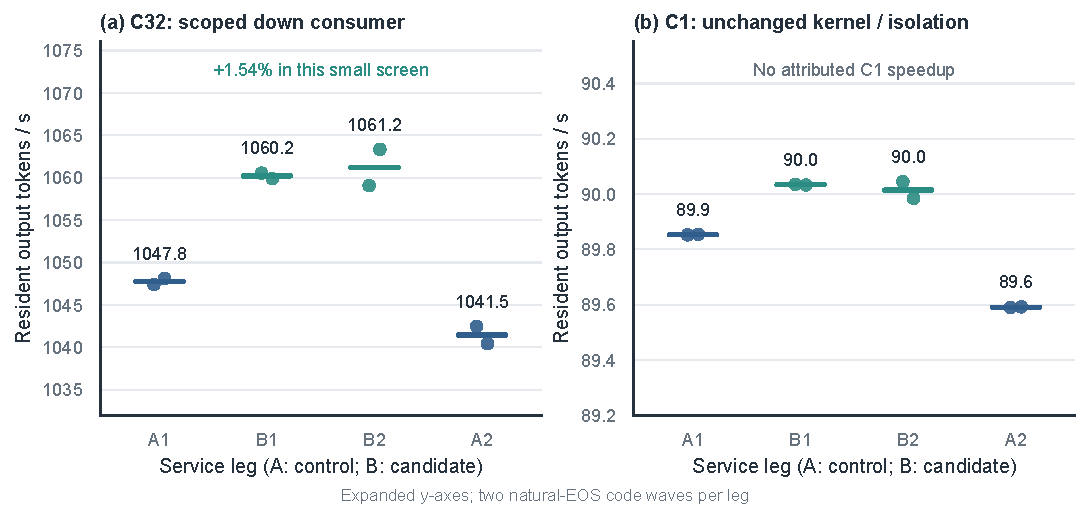
\includegraphics[width=\textwidth]{figures/down_consumer_abba.pdf}
  \caption{Default-off down-consumer pilot, expanded y-axes. Dots are the two
  measured waves per leg; short bars mark their median. C1 never executes
  the candidate and is a negative-control scope check.}
  \label{fig:consumer-abba}
\end{figure}

\section{Historical speculative decoding: separate evidence}
\label{sec:spec-history}

The latest native-AR matrix deliberately excludes DSpark. We retain the
September 11 full-target result as historical evidence, not a claim that the
latest merged DSpark service has been revalidated. This distinction also
prevents an earlier approximate-target speed from becoming a recovery target.

\subsection{Why the historical TP4 1.5k result is not a strict baseline}

In the old anchor-only/compact routed-MoE path, C32 with three draft positions
produced M128 target rows, but only 32 anchor rows executed the full routed
expert branch. Non-anchor rows omitted routed experts. Keeping stored weights
unchanged did not preserve the full target function at those positions.
Consequently, approximately 1.5k resident tok/s from that path is an
\emph{approximate-target} result. It cannot be presented as native AR or
lossless full-target verification, even if an early France answer passed.

M128 is a row count, not inherently speculative: native C128 would also
produce M128, whereas native C32 normally produces M32. Padding C32 to 128
does not compute three useful future AR positions for free. The new native
down-consumer pilot therefore tests actual M32 without reintroducing DSpark.

\subsection{Strict TP8 MHC fusion checkpoint}

The September 11 trial preserved all target experts, original weights,
TP-synchronized draft/accept decisions, a 1M logical pool, and gamma three.
It used 32 real-code requests, 512 outputs with \texttt{ignore\_eos}, and
chunk 2304. Four measured resident windows per family gave:

\begin{table*}[tp]
  \centering
  \caption{Historical full-target DSpark only; not a current AR comparison.
  Acceptance and throughput are reported in their original trial scope.}
  \label{tab:dspark-history}
  \begin{tabular}{@{}lrrr@{}}
    \toprule
    Family & Resident tok/s & Mean accept length & Relative to control \\
    \midrule
    Control & 1073.16 & 2.687 & --- \\
    Fusion + FP32 mixing & 1127.48 & 2.732 & +5.06\% \\
    Fusion + FP16 mixing & 1142.26 & 2.698 & +6.44\% \\
    \bottomrule
  \end{tabular}
\end{table*}

FP32 mixing was selected historically. The FP16--FP32 mean gap of about
1.31\% was smaller than the observed FP16-family range of 2.5\%, their ranges
overlapped, and only four windows per family were available. FP16 also had a
larger component perturbation and the trial's single observed semantic
degeneration. These observations motivate the conservative choice, not a
statistical proof that either rounding variant is universally safer.

\begin{figure*}[tp]
  \centering
  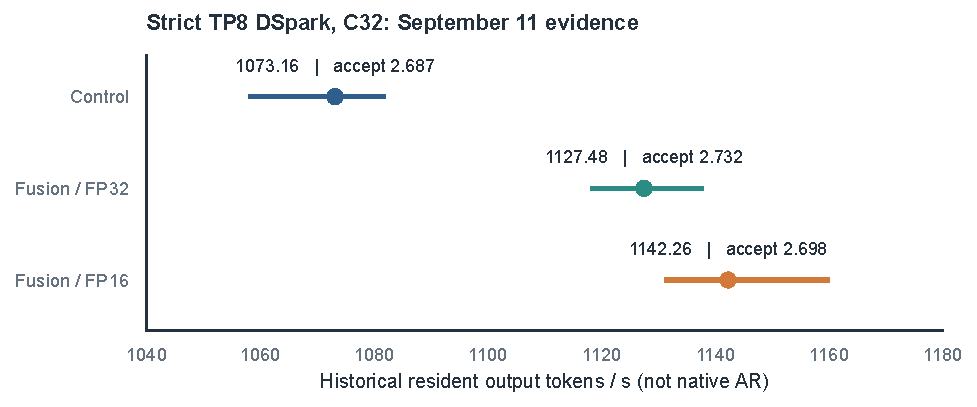
\includegraphics[width=.90\textwidth]{figures/strict_dspark_history.pdf}
  \caption{Historical strict DSpark family means with the ledger's rounded
  observed min/max ranges, not confidence intervals. Native AR, natural EOS,
  and the September 14 C32 pilot are deliberately not plotted on this axis.}
  \Description{Historical strict DSpark means are 1073.16 for control, 1127.48 for FP32 fusion, and 1142.26 for FP16 fusion; intervals are rounded observed ranges, not confidence intervals.}
\end{figure*}

\subsection{Acceptance, timing, and drift}

For concurrency $C$, average committed tokens per request $a$, and complete
speculative step time $T_{\mathrm{SD}}$, useful throughput is
$Ca/T_{\mathrm{SD}}$. It exceeds native AR only if
$T_{\mathrm{SD}}/T_{\mathrm{AR}}<a$. Larger verification batches expand expert
work and may not amortize draft cost. Acceptance alone is not a speed metric.

In the historical trial, chunked admission ramped the active batch through
several sizes before all requests were resident. Controls differed from
themselves on most complete output sequences. Such changes in batching and
numerical execution confound attribution from final hashes; they do not prove
that all other numerical or synchronization risks are absent. Most flagged
dot tails were forced continuation after EOS, distinct from genuine semantic
repetition. This motivated the natural-EOS protocol used in the new AR matrix.
The 1127.48 figure must not be divided by the new 1044.32 AR figure to claim a
matched speculative speedup: output policy, input mixture, chunking and date
differ. A fresh matched AR/strict-DSpark experiment remains outside this update.


\section{Measurement methodology}
\label{sec:method}

\subsection{Resource and metric controls}

Every GPU experiment begins with:

\begin{lstlisting}[language=bash]
amd-smi process --json
\end{lstlisting}

Launchers compare GPU owners with their recorded service PID, birth time, command, and descendants before each test. They refuse unrelated GPU owners and terminate only the owned test process tree. The native campaign verifies the original model path, TP size, speculative algorithm being absent, actual graph row counts, and KV pool size. Logged flags alone are not proof that a specialized kernel was selected.

Early experiments used NUMA node 1 because the host had a known node-0 memory fault, independent of MI250 or SGLang. The operator subsequently reported that fault repaired. The September 13--14 launcher uses NUMA interleaving across the host; it does not retain the old node-1-only policy. This report does not claim a new hardware-health diagnosis.

Approximately five-second AMD-SMI observations recorded a peak of 45,773/65,520 tool-reported MB per GCD (69.86\%) during the final decode observations. Separate large-prefill observations reached about 82.60\%; prefill coverage was incomplete. These are sampled observations, not exact allocator peaks, and \texttt{mem\_fraction\_static=0.96} is a budgeting setting rather than a claim of constant 96\% utilization. Logical KV capacity, allocated storage, graph/workspace memory, and occupied context are different quantities.

\subsection{Timing definitions and aggregation}

Let $f_i$ and $e_i$ be the first and last streamed-token timestamps of request $i$, and $n_i(t)$ its cumulative output count. The common resident interval is
\begin{equation}
  t_s=\max_i f_i,\qquad t_e=\min_i e_i,\qquad
  R_D=\frac{\sum_i[n_i(t_e)-n_i(t_s)]}{t_e-t_s}.
\end{equation}
Only intervals with $t_e>t_s$ contribute. Multiple waves contribute token and duration sums within each formal round; the reported cell is the median of three round rates. This is streamed service wall time, not pure GPU timing. Whole-wave HTTP rate instead divides all completed output tokens by wave start-to-last-response time. Prefill rate divides all prompt tokens by wave start-to-last-first-token time, including admission and first-token overhead. The two-column P/D matrix does not describe disaggregated serving.

Candidate comparisons use the order

\begin{equation}
  A_1 \rightarrow B_1 \rightarrow B_2 \rightarrow A_2.
\end{equation}

A1 and A2 use independently started control processes; consecutive B1/B2 legs can share one candidate process. This is stated per experiment, not represented as four independent starts. Explicit warmup files are excluded. Measured outliers remain in the formal three-round matrix. The small down-consumer pilot uses two fixed waves per leg and mean arm medians for its ABBA comparison. No statistical confidence interval is inferred from these small samples. Earlier trimmed-mean or short-probe protocols retain their original labels.

The initial request can trigger compilation even after another shape was warm. The new corpus includes 511/512-token rows; different admission groups exposed M8190/M8191 below the M8192 CK selector. Object timestamps and Ninja records associated four builds totaling about 23.1 s with one slow wave. This evidence explains that cold-shape event, not all HTTP variability. Runtime-M repair already removed one small-prefill specialization problem, but remaining exact-M tails are an open latency risk. Generated IDs, raw stream samples, finish reasons, input hashes, and cold/warm separation are retained outside temporary directories.

\subsection{Correctness hierarchy}

\begin{enumerate}[leftmargin=2em]
  \item Kernel level: elementwise bitwise equality, maximum absolute error, relative L2, and cosine similarity.
  \item Layer level: router top-k, stage 1, activation, stage 2, and rank-local sum.
  \item Model level: independent decoding of completion-only IDs, semantic sentinels, and matched fixed-input/logit checks. France is a short sanity check, not a quality benchmark.
  \item Attribution level: batch shapes, admission, prefixes, physical cache state, and numerical path must be controlled before comparing whole output hashes. Greedy divergence alone cannot identify the faulty operator.
  \item Remaining coverage: broad teacher-forced cached-versus-recompute tests at compression/window/indexer boundaries and filled-long-context quality evaluation. Existing local fixtures are not universal coverage.
\end{enumerate}

\section{Rejected or reverted directions}

The following observations are historical, shape/configuration-specific results from the experiment ledger. They do not prove a general algorithm or ISA instruction is unusable, and were not all rerun during this report update. Component timing is never substituted for a service-level win.

\begin{longtable}{@{}p{0.27\textwidth}p{0.22\textwidth}p{0.44\textwidth}@{}}
  \caption{Important negative results and their implications.}\label{tab:negative}\\
  \toprule
  Direction & Result & Conclusion \\
  \midrule
  \endfirsthead
  \toprule
  Direction & Result & Conclusion \\
  \midrule
  \endhead
  CKTile KSPLIT=2/4 & Approximately 25/22 tok/s or lower & Split-K reduction and CTA pressure do not suit BS1 small-M MoE. \\
  AsyncLL / SDMA Mori & Approximately 20--49 tok/s & The current low-latency transport does not shorten the critical path. \\
  Offline FP4-to-INT8 expansion & Gate 7.23$\rightarrow$10.45 ms & Doubled weight traffic costs more than removing online unpack. \\
  CK BF16 router instances & Approximately 86.7--98.6 $\mu$s & Slower than stable torch/rocBLAS; not integrated. \\
  Simple LDS BF16 MFMA router & Approximately 0.43--0.52 ms & Barrier and bank/layout costs dominate. \\
  32$\times$32 INT8 MFMA gate & Best approximately 7.87 ms & 165 VGPR plus 32 KiB LDS collapses occupancy. \\
  Full prefill CUDA Graph & Capture succeeds; replay faults & Prefill metadata addresses are not capture-stable. \\
  One-CTA/token HIP mHC prefill & Approximately 28\% slower & Scalar FMA cannot replace the current decomposition by launch reduction alone. \\
  RCCL in place of peer-read AR & TTFT 0.679$\rightarrow$0.711 s & Reduce collective boundaries instead of substituting RCCL. \\
  BF16 down partial & Approximately 0.8\% micro gain with broad value changes & Insufficient benefit; retain FP32 partials. \\
  \bottomrule
\end{longtable}

\section{Serving, memory, and agent integration}

\subsection{Reproducible configuration, not a live deployment}

The earlier four-GCD deployment allocated a 560,896-token pool and exposed graph tiers 1/2/4. The latest tested configuration instead uses TP8/EP1, pool 1,048,576, memory fraction 0.96, seven decode tiers, admission 16 for prefill, and chunk 36,864. All benchmark services were shut down after testing. No current endpoint availability, LAN exposure, or continuously running GPU workload is claimed.

The documented launcher starts a loopback service on port 30021 only when explicitly invoked. A user should discover its served model ID before sending a chat request; the performance harness bypasses chat tokenization by supplying the frozen input IDs directly.

\begin{lstlisting}[language=bash]
curl http://127.0.0.1:30021/v1/models
curl http://127.0.0.1:30021/v1/chat/completions \
  -H 'Content-Type: application/json' \
  -d '{
    "model": "<served-model-id>",
    "messages": [{"role": "user", "content": "Hello"}],
    "max_tokens": 64
  }'
\end{lstlisting}

\subsection{Historical API and agent integration}

Earlier work implemented OpenAI-compatible model discovery, streaming chat, a separate optional system-prompt proxy, and tool-result round trips for DeepSeek Harness\cite{dsh}. Those endpoints were not part of the new performance measurements, and the proxy's availability is not revalidated here. No private host address or persona is needed to reproduce the benchmark.

The earlier parser configuration was:

\begin{lstlisting}
--tool-call-parser deepseekv4
--reasoning-parser deepseek-v4
\end{lstlisting}

Streaming/non-streaming tool-call checks were interface smokes, not throughput or model-quality measurements. Reproduction should use the archived launcher and input manifest rather than infer configuration from an old endpoint example.

\section{Remaining risks and next steps}

\begin{enumerate}[leftmargin=2em]
  \item \textbf{Capacity is not occupancy.} Fill the allocated 1M pool with controlled long contexts and verify quality, admission, sustained throughput, and exact memory peaks. Current measurements do not provide this evidence.
  \item \textbf{Numerical coverage.} Preserve deterministic Top-K membership/order, test real nonconstant scale layouts, and separate atomic/reduction-order variation from scheduling-dependent trajectories. Fixed-slot CK stage-2 reduction remains a possible experiment, not a measured gain here.
  \item \textbf{Cold-shape coverage.} Audit exact-M compilation keys, prewarm supported shapes, and report cold/restart/warm TTFT independently. Do not hide latency outliers inside resident-only speed claims.
  \item \textbf{Indexer work.} Active-query production and elimination of full logits materialization are distinct from the accepted trivial-row and empty-tile skips. A historical M128 query-row partition saved about 9.7 microseconds in projection but required about 37 microseconds for optimized index exchange, so it was not integrated. Long-context opportunities require a new matched profile.
  \item \textbf{Controlled comparisons.} A matched current TP4/TP8 matrix and a fresh strict-DSpark regression remain unfilled evidence gaps. The current update ran neither; unavailable temporary artifacts are not reconstructed as invented measurements.
  \item \textbf{Deployment decision.} The C32 consumer remains opt-in after a small positive screen. Broader request mixtures and context ranges are required before changing a global default. The C1 isolation result is not another kernel optimization.
\end{enumerate}

\section{Conclusion}

The expanded study combines historical TP4 correctness recovery with a fresh single-instance TP8 evaluation. The formal native-AR matrix reaches 87.60 output tok/s at C1, 1044.32 at C32, and 1334.24 at C64, with 4.68--5.27k input tok/s on separate 8K prefill waves and a 1M allocated logical pool. Matched ABBA tests isolate two important changes: removing work on empty indexer tiles and restoring a missing C1 specialization. A later consumer-fusion screen adds a small 1.54\% resident gain at C32 without changing the C1 kernel.

The engineering evidence emphasizes stored-format/execution mismatch, small per-expert matrices, redundant work, specialization reachability, and fixed synchronization boundaries. It does not provide a hardware-counter roofline proving a single universal bottleneck. Keeping native AR, strict speculation, approximate targets, HTTP latency, and resident throughput separate is as important as the kernel work itself. The final deliverable is an auditable configuration and evidence archive, not a claim of universal bitwise equivalence or a completed million-token quality benchmark.

\appendix

\section{Key checkpoints}

\begin{longtable}{@{}p{0.20\textwidth}p{0.72\textwidth}@{}}
  \toprule
  Commit & Content \\
  \midrule
  \commit{505b3373794a} & Initial gfx90a/ROCm enablement \\
  \commit{caf80718cf} & CKTile FP4 expert W2 output-order repair \\
  \commit{9140c03605} & Correct TP-only 60 tok/s route \\
  \commit{b097d228c2} & Native router decode optimization \\
  \commit{ea519e2e0f} & Routed-MoE prefill MFMA \\
  \commit{6680714cf8} & Sparse-prefill wave reduction \\
  \commit{6547c5b063} & M2048 64-row expert block; long-prefill gain of 5.6\% \\
  \commit{85ab1a40c5} & DSV4 reasoning and tool parser wiring \\
  \commit{94d630a47c} & Full-endpoint OpenAI client compatibility \\
  \commit{b00a4e11cf} & Historical TP4 tree reproduced at 74.018 HTTP tok/s median on September 6 \\
  \commit{137170e367} & TP8 large-prefill migration with corrected scale interpretation \\
  \commit{9edb8ecdde} & Historical strict-DSpark FP32 MHC fusion profile (not the latest AR matrix) \\
  \commit{c224e9c1ce} & Fresh-start unified-V4 pool/metadata integration repair \\
  \commit{3d73a75923} & Formal seven-tier native P/D archive and C1 GEMV restoration \\
  \commit{fb2e39fca9} & Default-off native C32 down-consumer pilot and C1 isolation \\
  \bottomrule
\end{longtable}

\section{Reproducible report build}

\begin{lstlisting}[language=bash]
cd reports/gfx90a-dsv4
python generate_figures.py
make check
make
make arxiv
\end{lstlisting}

The report uses pdfLaTeX with TeX-distributed Helvetica-compatible Type 1 fonts. Figures embed Arial and retain only left/bottom spines. Normal compilation does not require Python, Biber, BibTeX, shell escape, host font discovery, or a GPU. Python/Seaborn is needed only to regenerate figures from the frozen data. The source bundle includes all TeX inputs and pre-generated PDF figures, excluding the compiled article and auxiliary files. A local build from the extracted bundle is verified after references stabilize; this is not a claim of testing arXiv's remote service.

\section{Evidence provenance and open gaps}

The report-local \texttt{data/results.json} freezes all three formal rounds per cell, ABBA samples, input/source hashes, and evidence archive identifiers. \texttt{prepare\_report\_data.py} explicitly refreshes that snapshot from repository evidence; normal builds do not access parent directories. Latest formal evidence is under \path{.agents/experiments/dsv4_tp8_revalidation_20260913/}; the consumer pilot is under \path{.agents/experiments/dsv4_tp8_ar_down_consumer_20260914/}. The formal archive contains 278 verified files; the pilot contains 92. Their complete SHA256 values are retained with the report data. These checks protect the recorded artifacts, not unrecorded measurements or the full checkpoint weights.

Historical TP4 records and the September 11 DSpark table are ledger evidence with explicitly different protocols. Older temporary full-matrix files were unavailable during this update, so no missing TP4 concurrency cells are filled from memory. Public source excerpts are fixed at repository revision \commit{54b93c45c2}; a source-path list may be longer than the text retained after prompt trimming. Neither source-review prose nor a simple France question measures general code correctness. Dataset-specific performance should not be mistaken for a model-quality benchmark or a matched comparison against another hardware platform.

\begin{thebibliography}{99}
  \raggedright
  \bibitem{dsv4card}
  DeepSeek-AI.
  \newblock \emph{DeepSeek-V4-Flash Model Card}.
  \newblock \url{https://huggingface.co/deepseek-ai/DeepSeek-V4-Flash}, 2026.

  \bibitem{amdisa}
  Advanced Micro Devices, Inc.
  \newblock \emph{AMD Instinct MI200 CDNA2 Instruction Set Architecture}.
  \newblock \url{https://www.amd.com/content/dam/amd/en/documents/instinct-tech-docs/instruction-set-architectures/instinct-mi200-cdna2-instruction-set-architecture.pdf}.

  \bibitem{dsv4report}
  DeepSeek-AI.
  \newblock \emph{DeepSeek-V4: Towards Highly Efficient Million-Token Context Intelligence}.
  \newblock \url{https://arxiv.org/abs/2606.19348}, 2026.

  \bibitem{dspark}
  X. Cheng et al.
  \newblock \emph{DSpark: Confidence-Scheduled Speculative Decoding with Semi-Autoregressive Generation}.
  \newblock \url{https://arxiv.org/abs/2607.05147}, 2026.

  \bibitem{cdna2}
  Advanced Micro Devices, Inc.
  \newblock \emph{AMD CDNA 2 Architecture White Paper}.
  \newblock \url{https://www.amd.com/content/dam/amd/en/documents/instinct-business-docs/white-papers/amd-cdna2-white-paper.pdf}.

  \bibitem{sglang}
  L. Zheng et al.
  \newblock \emph{SGLang: Efficient Execution of Structured Language Model Programs}.
  \newblock In \emph{Proceedings of NeurIPS}, 2024. \url{https://arxiv.org/abs/2312.07104}.

  \bibitem{vllm}
  W. Kwon et al.
  \newblock \emph{Efficient Memory Management for Large Language Model Serving with PagedAttention}.
  \newblock In \emph{Proceedings of SOSP}, 2023. \url{https://arxiv.org/abs/2309.06180}.

  \bibitem{dsv3}
  DeepSeek-AI.
  \newblock \emph{DeepSeek-V3 Technical Report}.
  \newblock \url{https://arxiv.org/abs/2412.19437}, 2024.

  \bibitem{megablocks}
  T. Gale et al.
  \newblock \emph{MegaBlocks: Efficient Sparse Training with Mixture-of-Experts}.
  \newblock In \emph{Proceedings of MLSys}, 2023. \url{https://arxiv.org/abs/2211.15841}.

  \bibitem{ck}
  AMD ROCm.
  \newblock \emph{Composable Kernel}.
  \newblock \url{https://github.com/ROCm/composable_kernel}.

  \bibitem{aiter}
  AMD ROCm.
  \newblock \emph{AIter: AI Tensor Engine for ROCm}.
  \newblock \url{https://github.com/ROCm/aiter}.

  \bibitem{dsh}
  DeepSeek-AI.
  \newblock \emph{DeepSeek Harness}.
  \newblock \url{https://github.com/deepseek-ai/deepseek-harness}.
\end{thebibliography}

\end{document}
